\section{Sharding}


En el ejercicio 7, nos piden experimentar con sharding.
Para esto decidimos tomar como base 3 mil registros de la tabla Competidor, y luego realizar la partición en 3 shards.\\
Generamos inserts cada 100 competidores, y registramos los resultado evaluados en los shard.\\

Al principio tuvimos problemas con este experimento, porque la tabla competidor que habiamos creado tenia como primary key el atributo Id(númerico), creabamos los 3 shards y luego insertabamos los datos, pero estos solo se acumulaban en uno de los shards. Luego de revisar la documentación, comprendimos que al crear los shards, la base de dato toma como valor de pivoteo, el valor medio de la primary key de los datos ya almacenados, y a partir de este distribuye los datos entre los shards.\\
En nuestro caso, el Id era númerico, consecutivo y creciente, por tanto luego de realizar la partición, los nuevos datos insertados se acumulaban en solo uno de los shards, dado que los ids nuevo eran mayores al valor medio que se eligió al inicio.\\
Entonces, para poder realizar el experimento correctamente, creamos la tabla sin asignarle la primary key, de manera tal de tener un clave alfanumérica y que la distribución sea en base a esta. A partir de ese momento, los datos vistos eran los esperados.\\
A continuación mostraremos un gráfico de los resultados:

\begin{center}
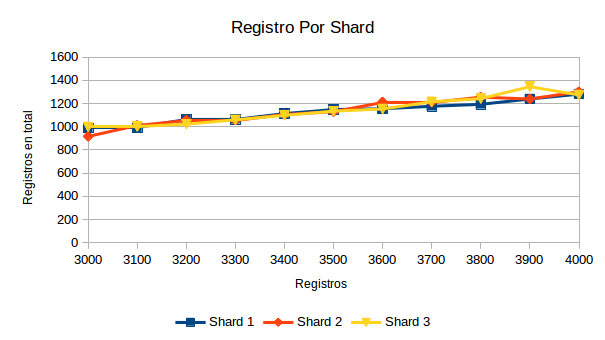
\includegraphics[width=13cm,keepaspectratio]{./imagenes/shard.png}\newline
\end{center}

Se puede ver que todos los shards tienden a tratar de acumularse en el mismo valor, por lo que podemos suponer que la distribución de los datos es uniforme. Creemos que esto se hace con el objetivo de no sobrecargar la base al realizar consultas o modificaciones.